\section{Appendix}
\label{sec:appendix}

% https://tex.stackexchange.com/a/210378
\renewcommand{\thefigure}{A.\arabic{figure}}
\setcounter{figure}{0}

\renewcommand{\thetable}{A.\arabic{table}}
\setcounter{table}{0}

Several large tables and figures are here for ease of reading.

\begin{figure}[t!]
    \centering
    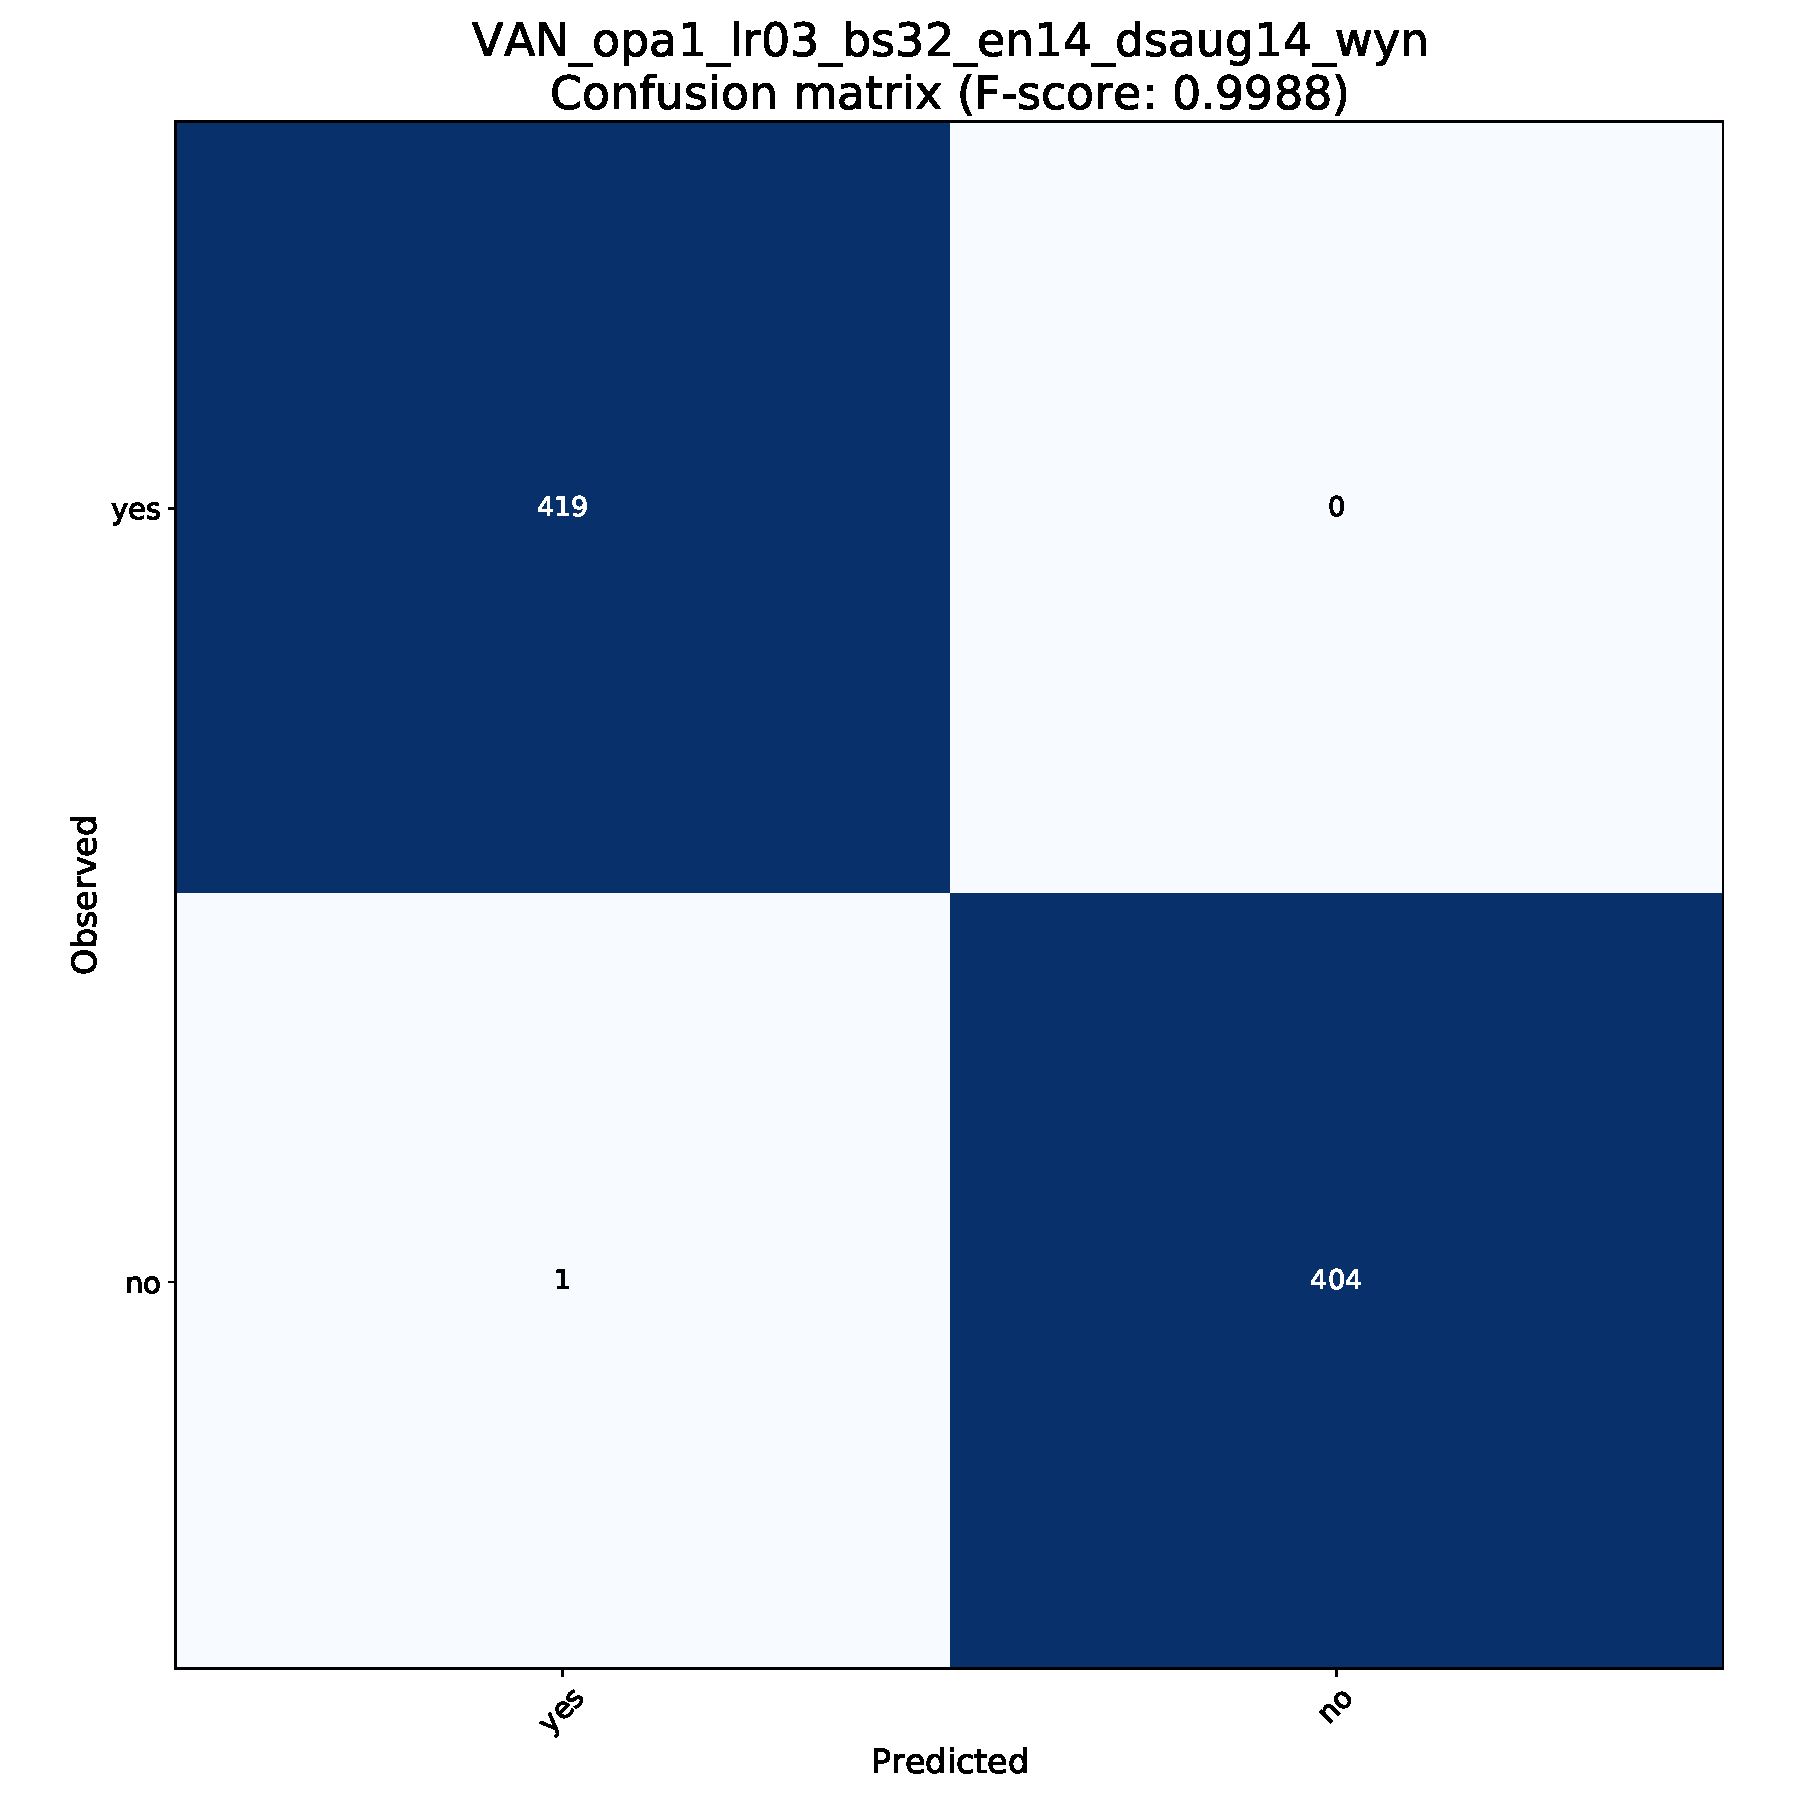
\includegraphics[width=0.9\linewidth]{VAN_opa1_lr03_bs32_en14_dsaug14_wyn_cm.pdf}
    \caption{Confusion matrix for VerticalAreaNet trained on the ``yes/no'' task.}%
    \label{fig:VAN_opa1_lr03_bs32_en14_dsaug14_wyn_cm}
\end{figure}

\begin{figure}[t!]
    \centering
    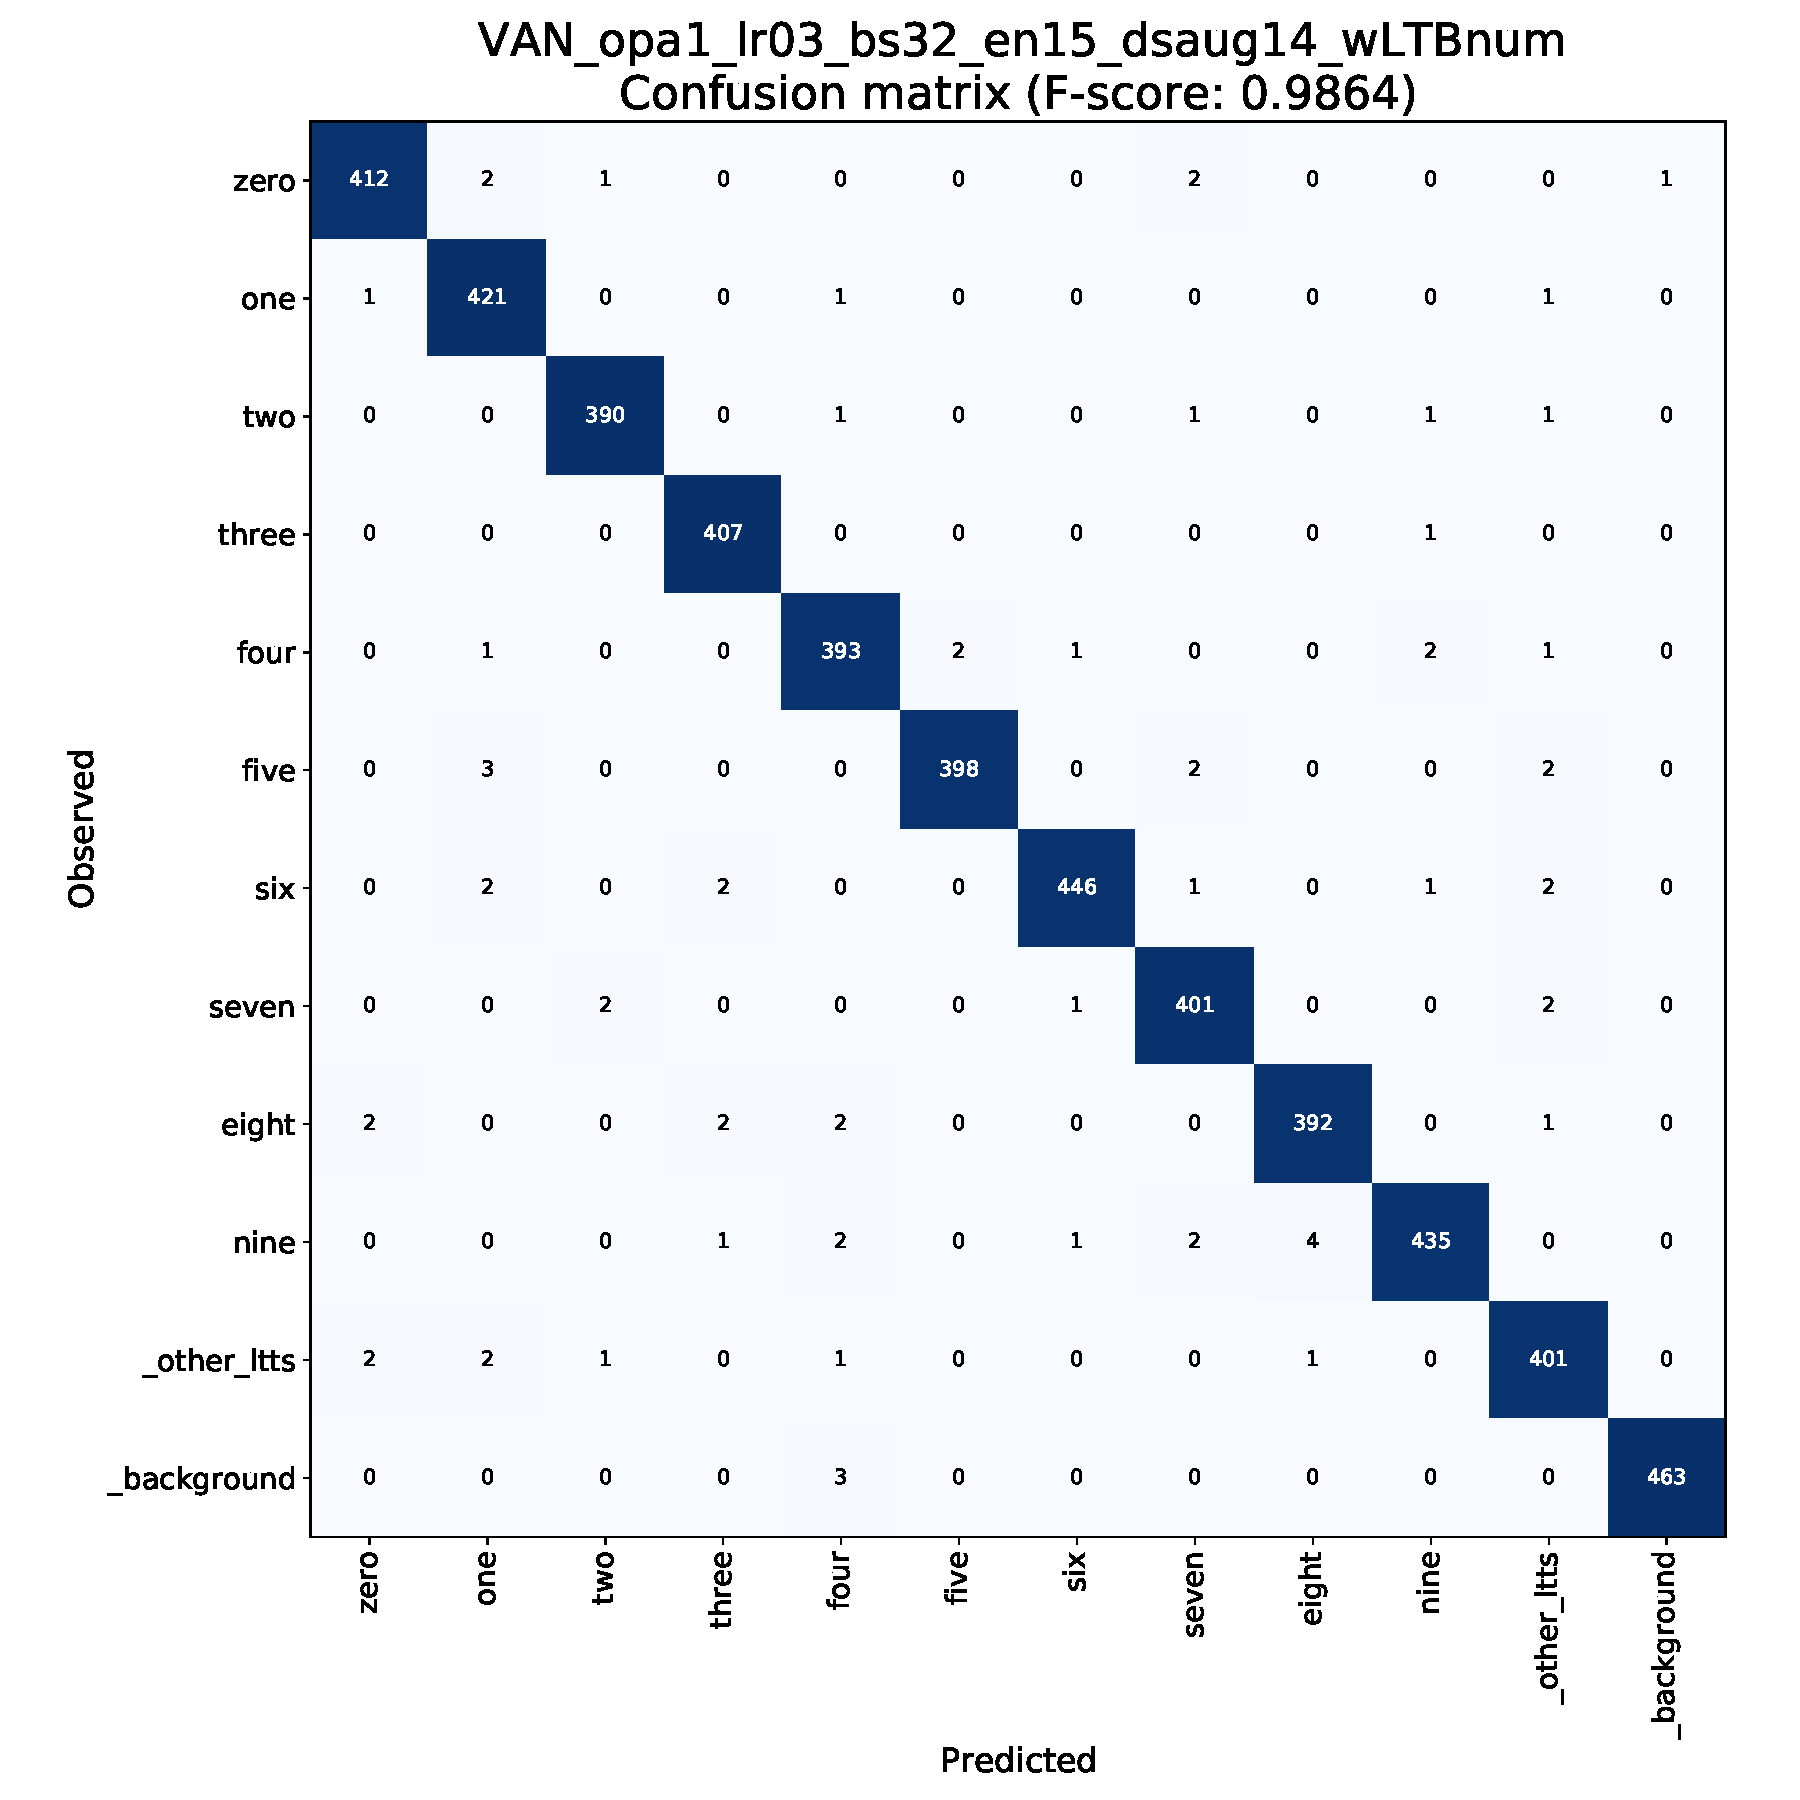
\includegraphics[width=0.9\linewidth]{VAN_opa1_lr03_bs32_en15_dsaug14_wLTBnum_cm.pdf}
    \caption{Confusion matrix for VerticalAreaNet trained on the ``LTBnum'' task, that contains
        the 10 number, one background conversation and one background noise classes.
    }%
    \label{fig:VAN_opa1_lr03_bs32_en15_dsaug14_wLTBnum_cm}
\end{figure}

\begin{figure*}[t!]
    \centering
    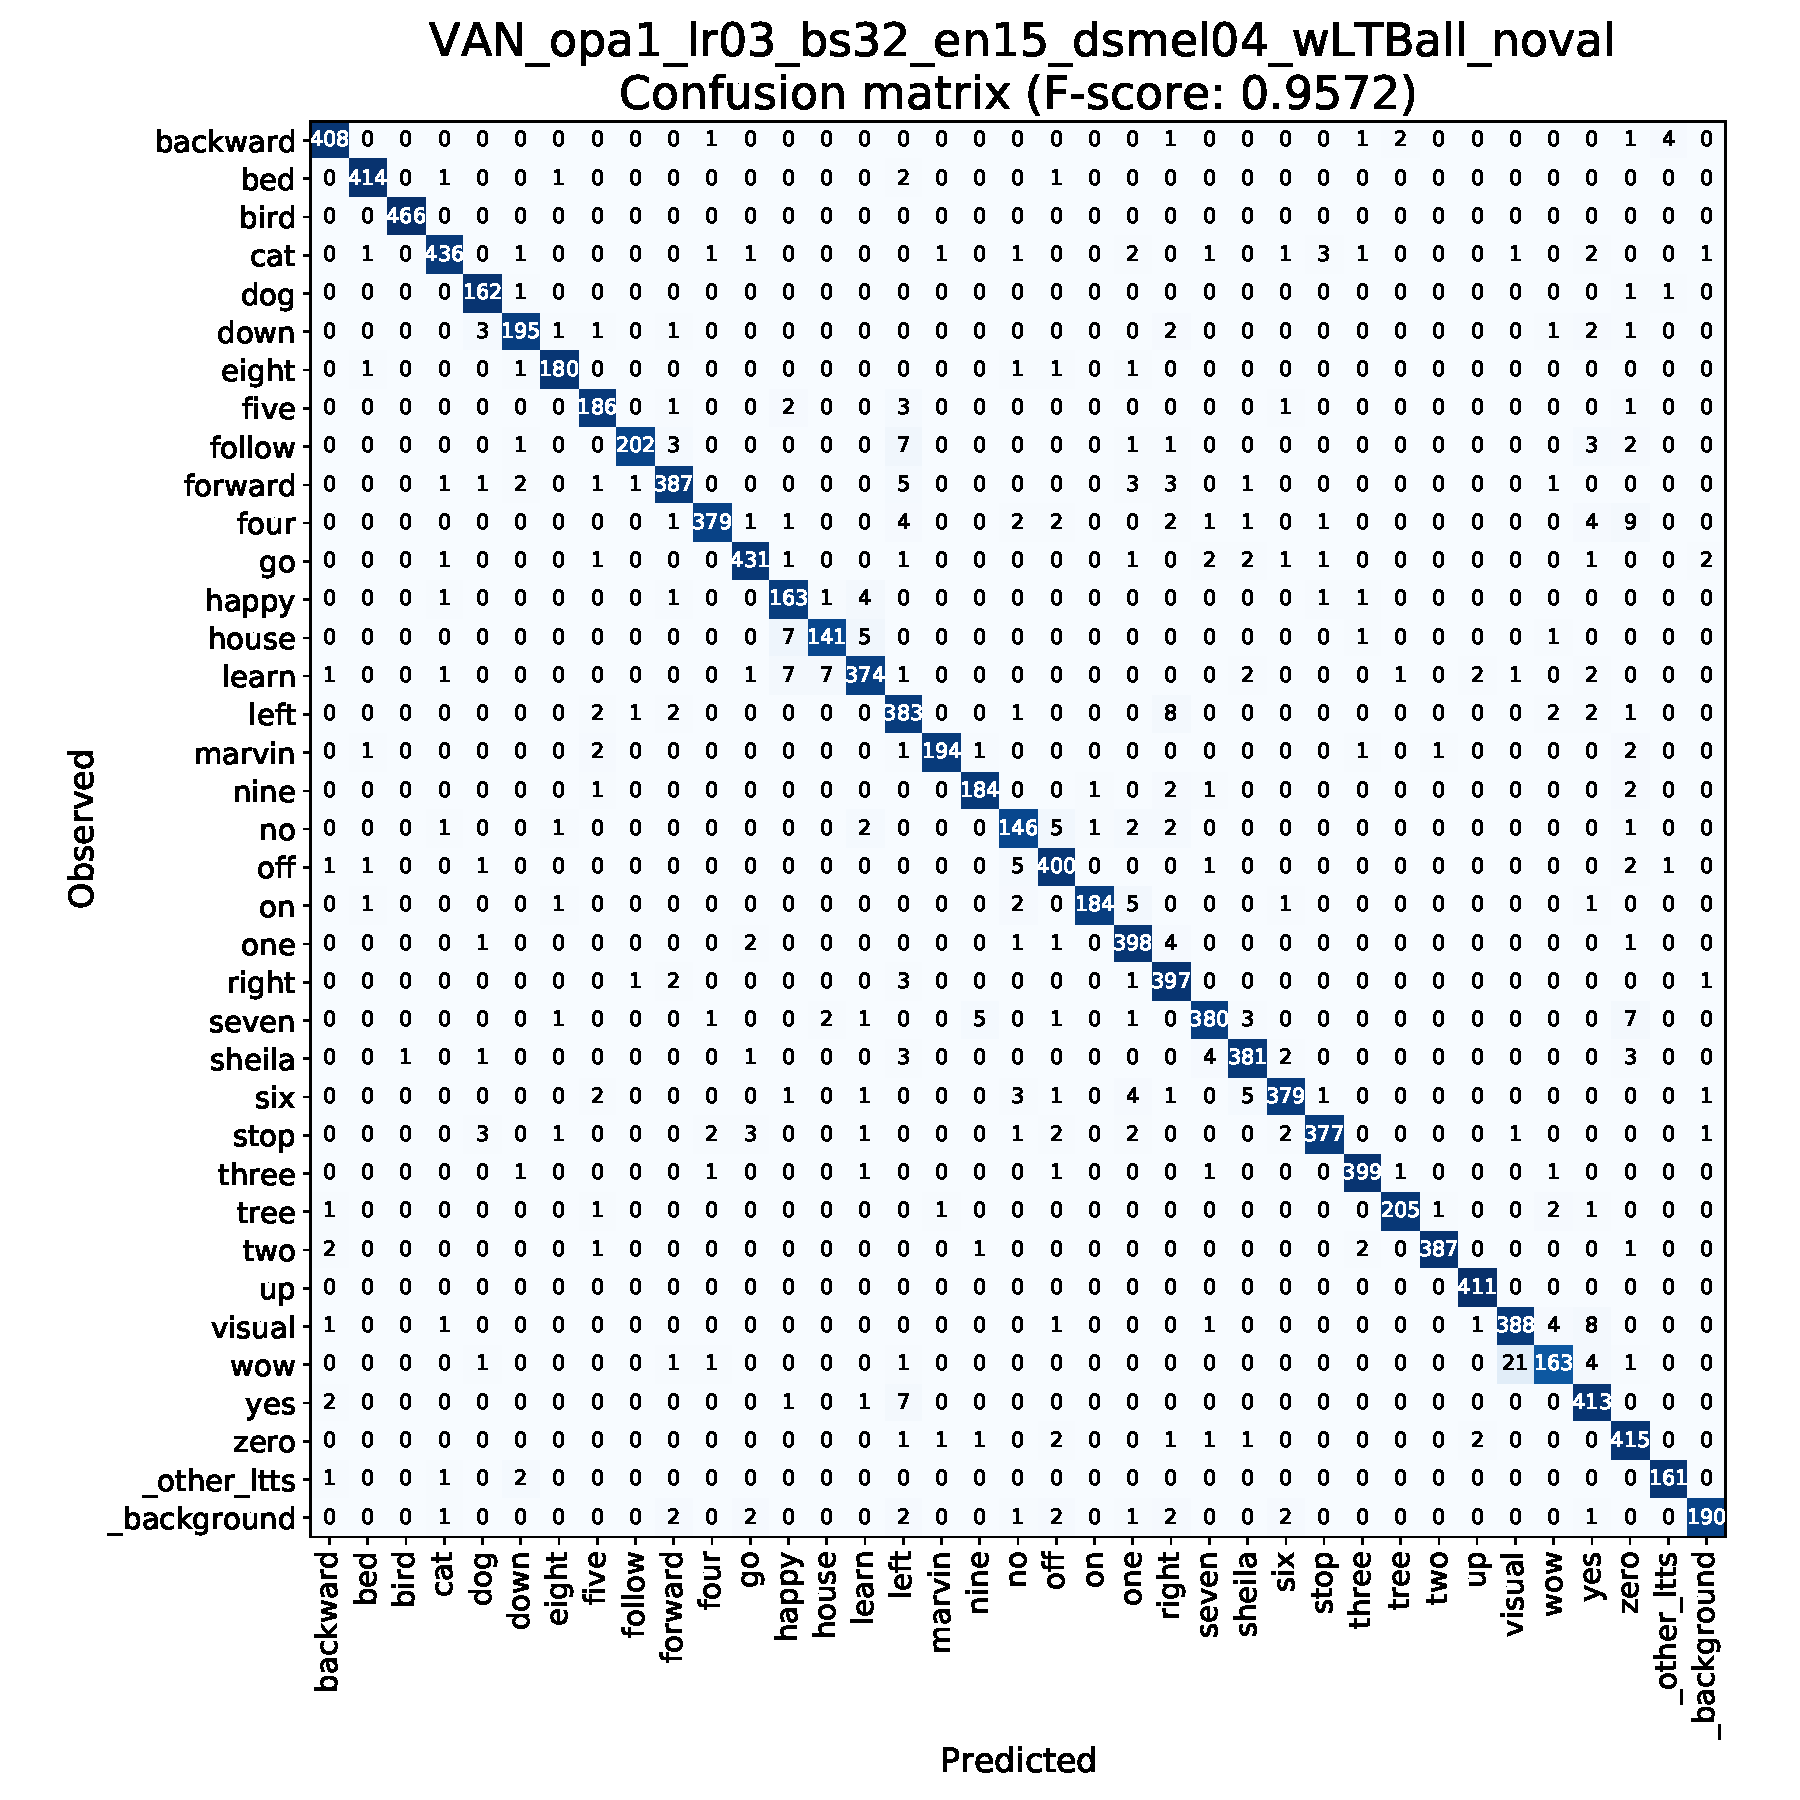
\includegraphics[width=0.9\linewidth]{VAN_opa1_lr03_bs32_en15_dsmel04_wLTBall_noval_cm.pdf}
    \caption{Confusion matrix for VerticalAreaNet trained on the ``LTBall'' task, that contains
        the 35 words, one background conversation and one background noise classes.
    }%
    \label{fig:VAN_opa1_lr03_bs32_en15_dsmel04_wLTBall_noval_cm}
\end{figure*}

\begin{figure*}[t!]
    \centering
    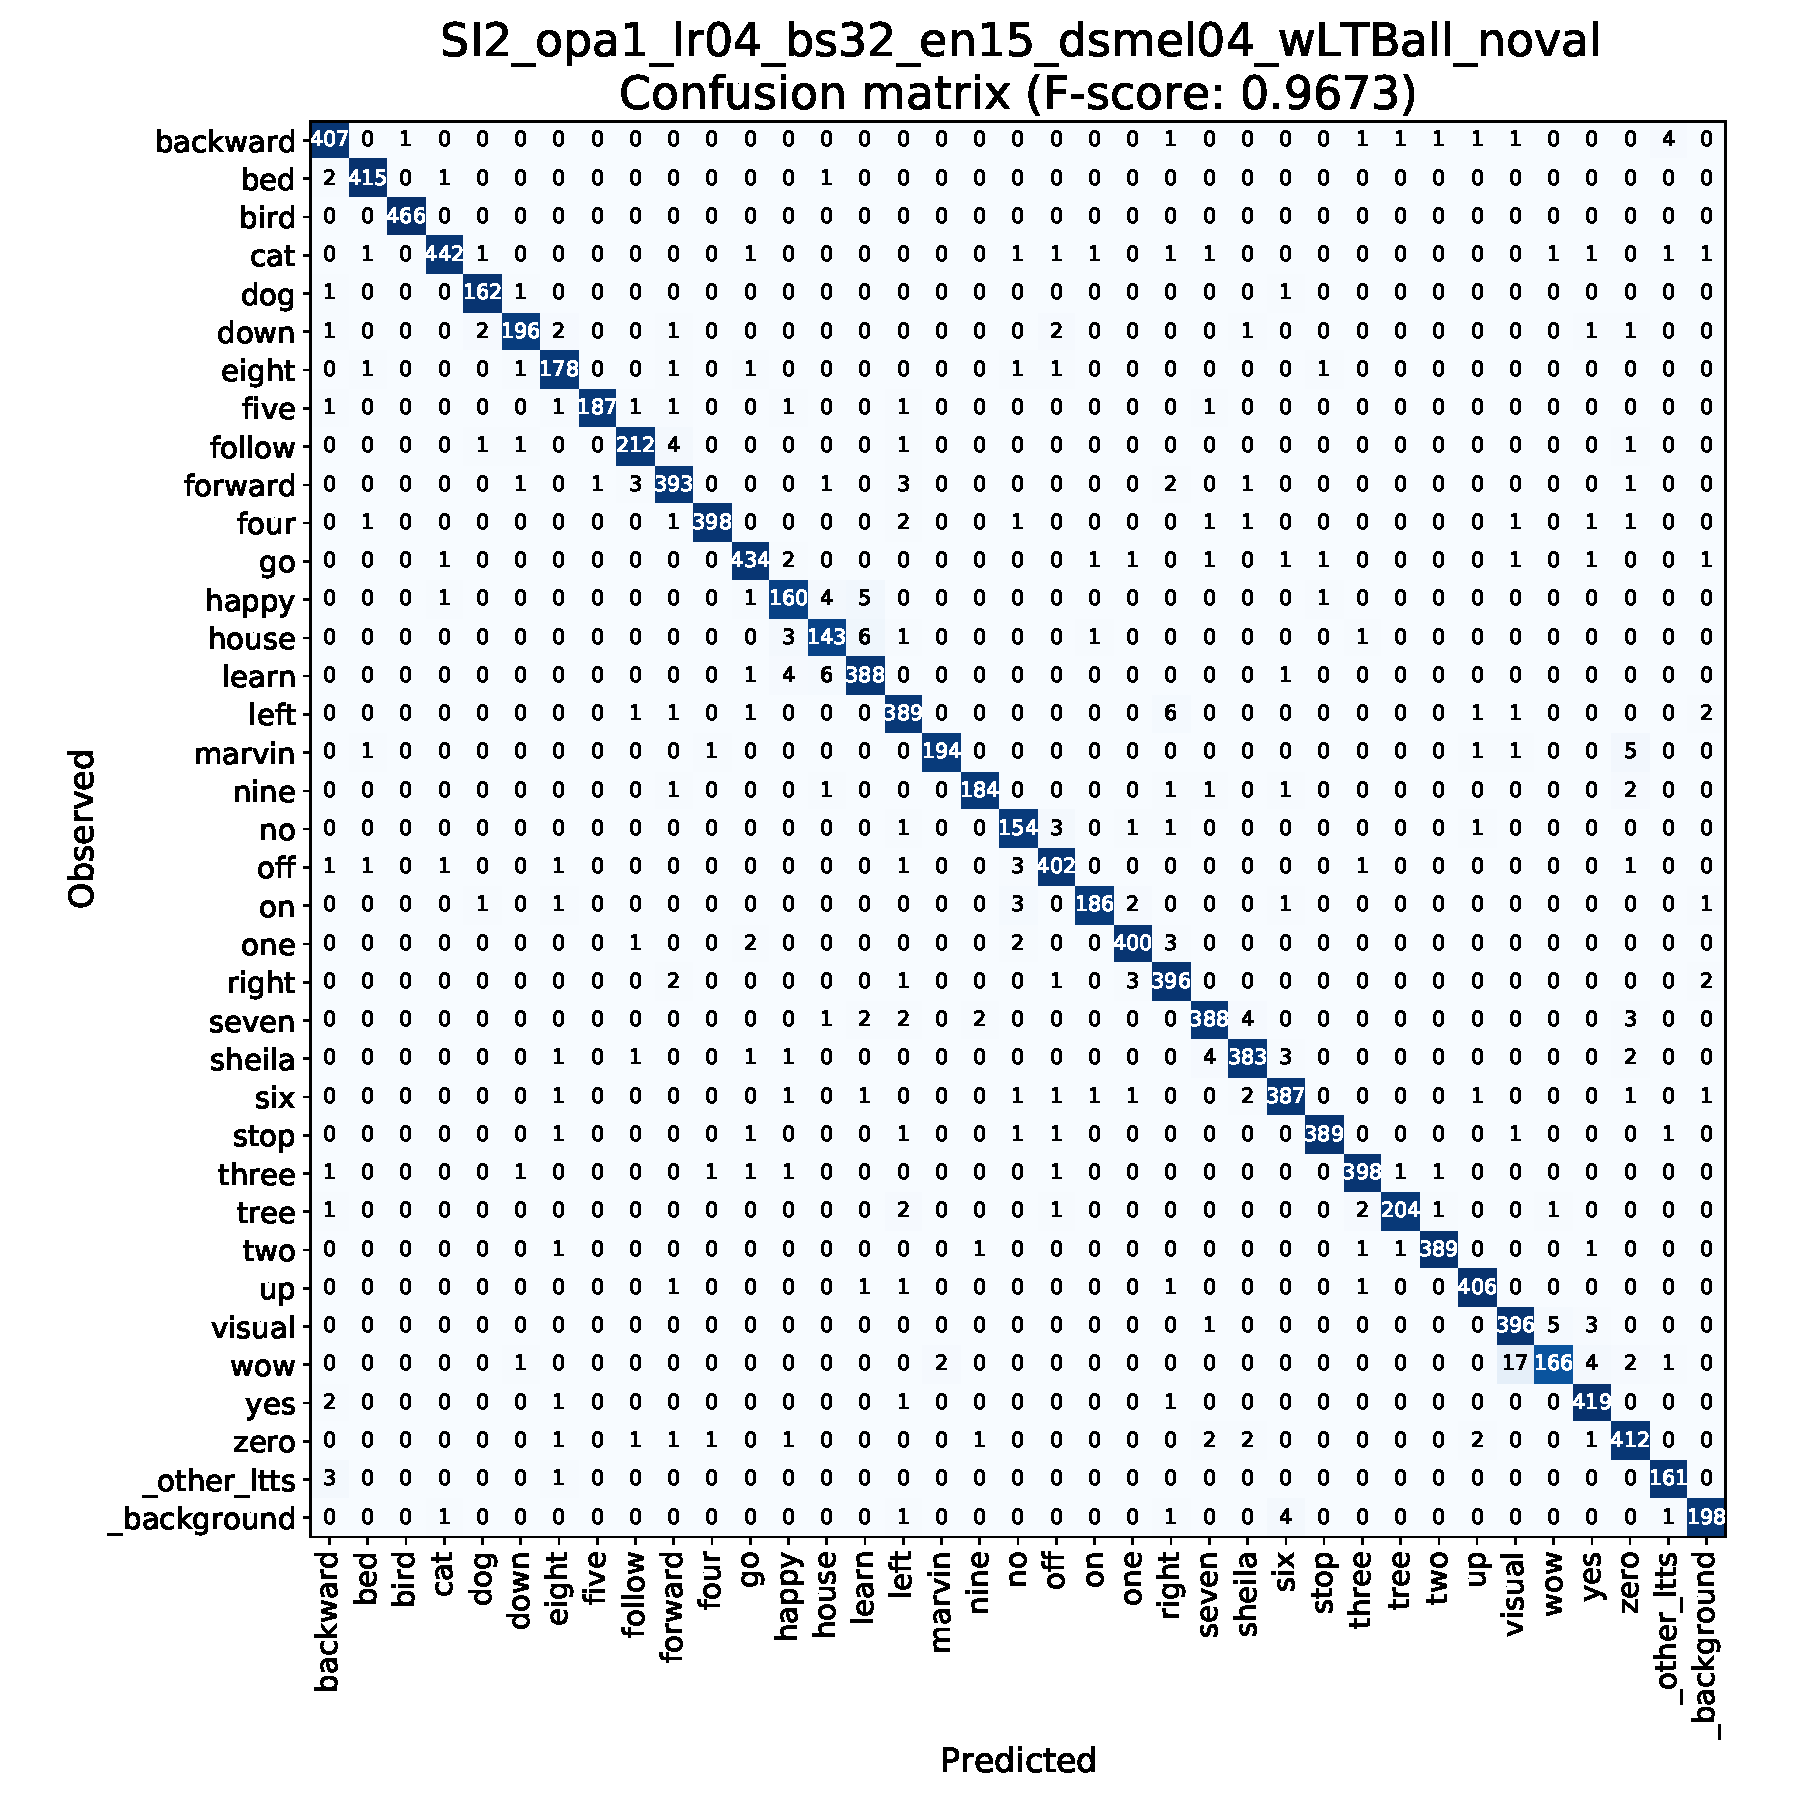
\includegraphics[width=0.9\linewidth]{SI2_opa1_lr04_bs32_en15_dsmel04_wLTBall_noval_cm.pdf}
    \caption{Confusion matrix for SimpleNet2 trained on the ``LTBall'' task, that contains
        the 35 words, one background conversation and one background noise classes.
    }%
    \label{fig:SI2_opa1_lr04_bs32_en15_dsmel04_wLTBall_noval_cm}
\end{figure*}

\begin{figure*}[t!]
    \centering
    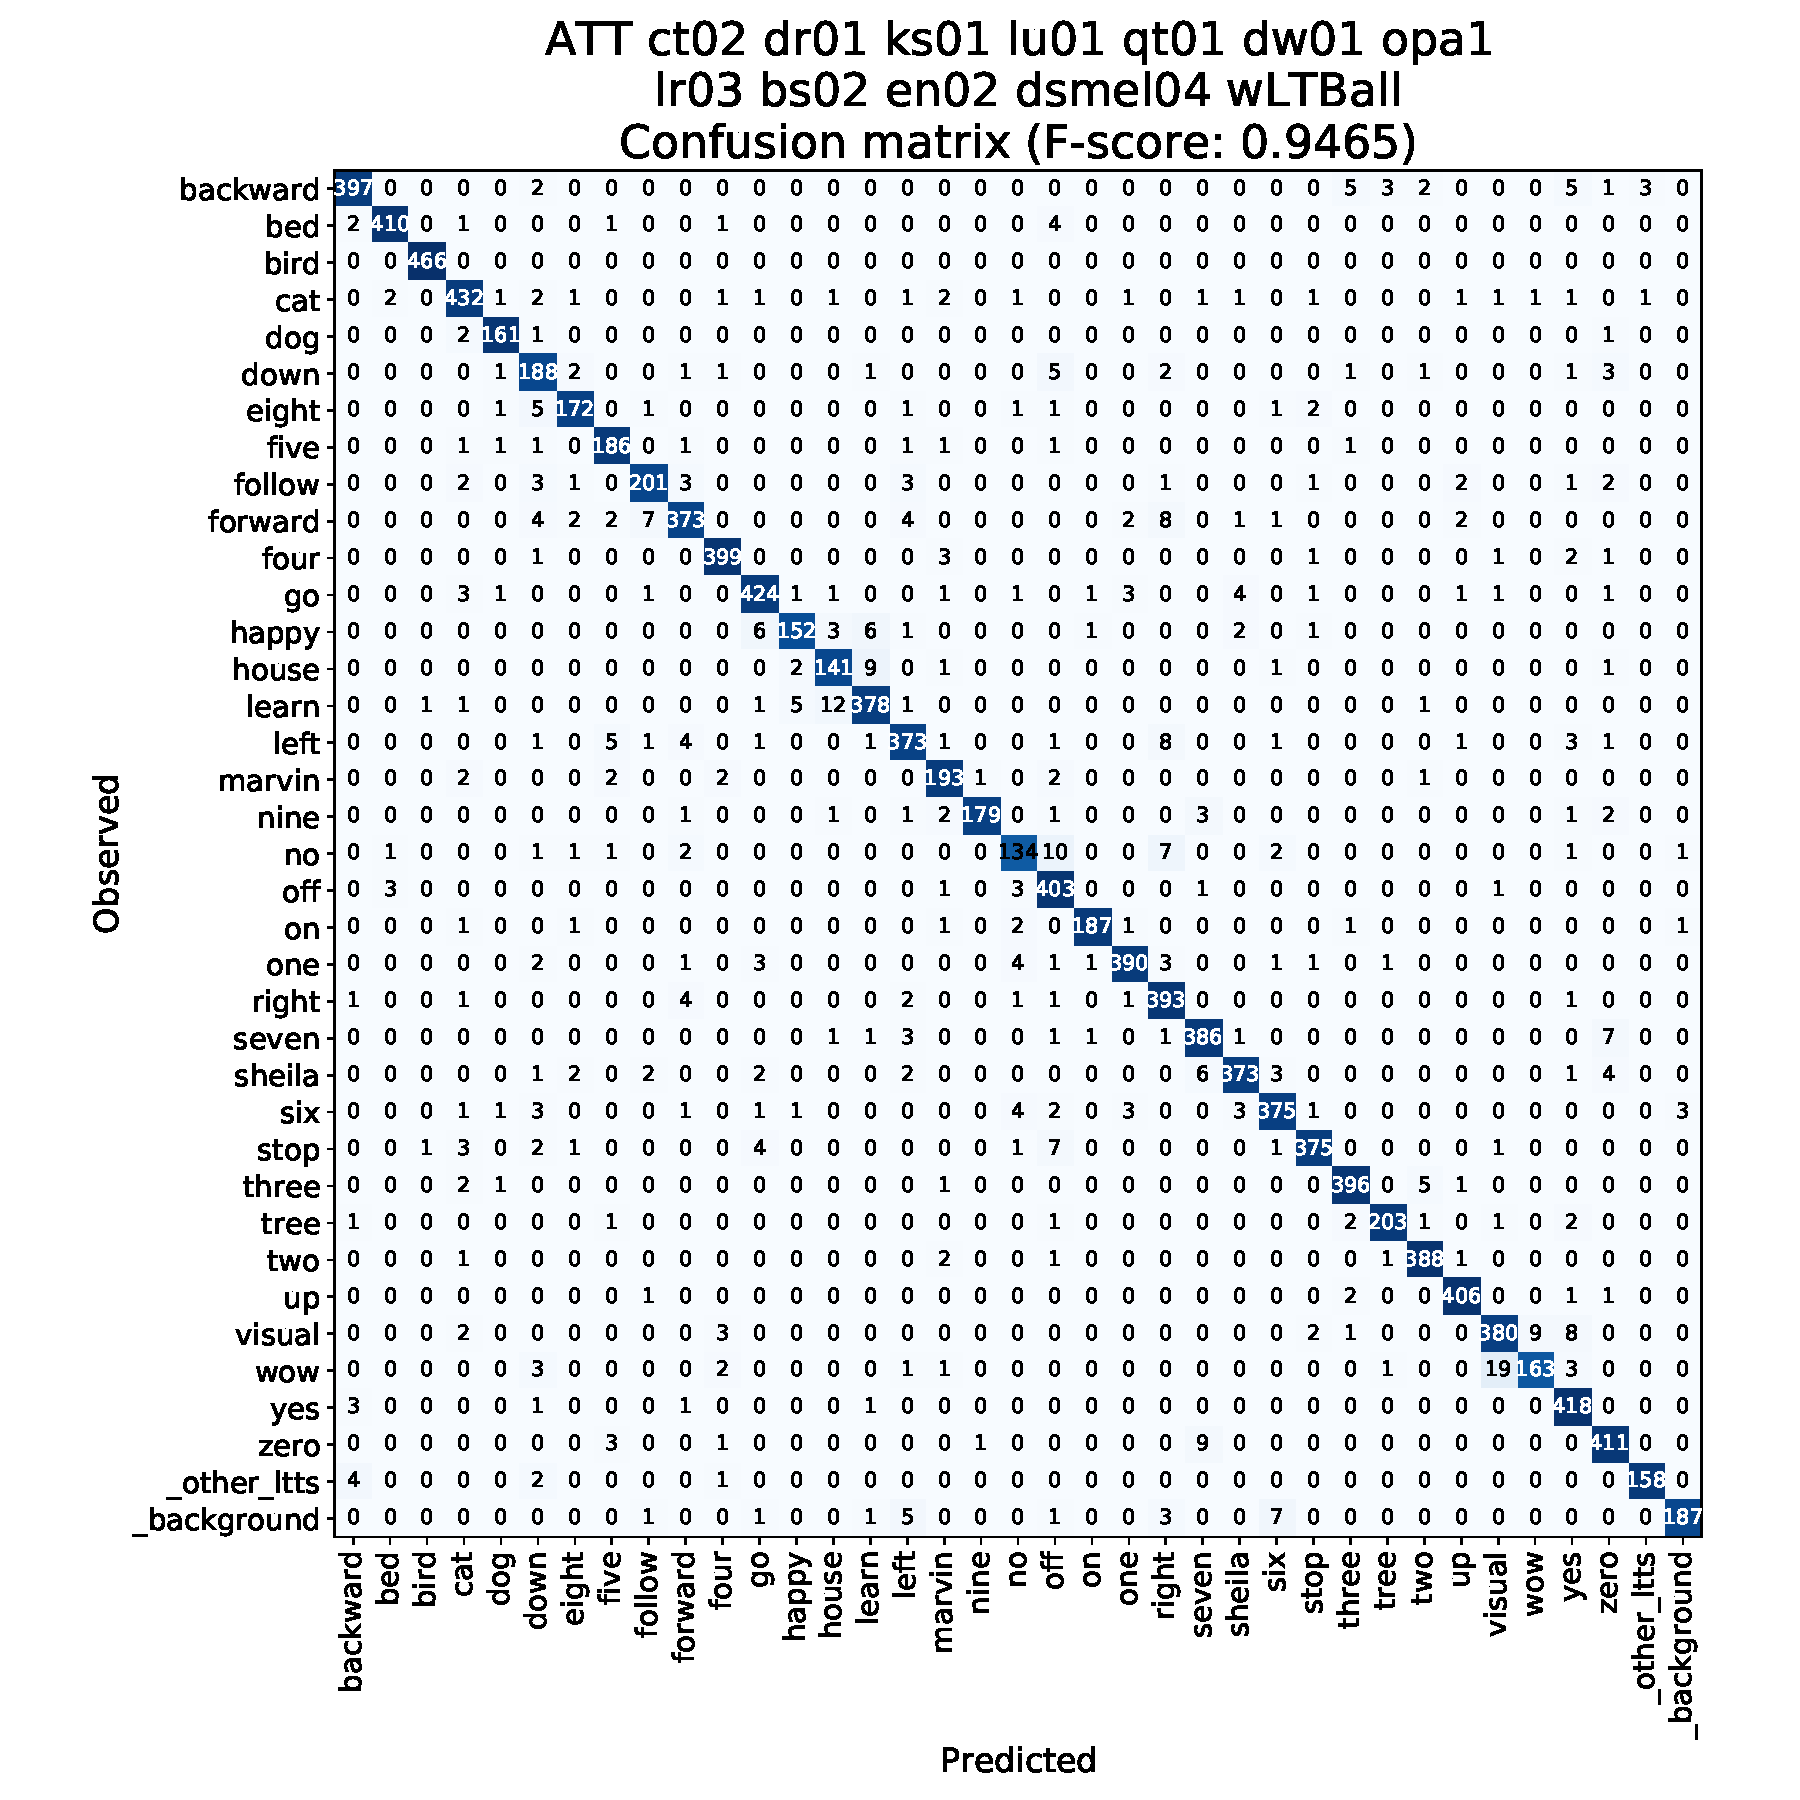
\includegraphics[width=0.9\linewidth]{ATT_ct02_dr01_ks01_lu01_qt01_dw01_opa1_lr03_bs02_en02_dsmel04_wLTBall_cm.pdf}
    \caption{Confusion matrix for LSTM+attention trained on the ``LTBall'' task, that contains
        the 35 words, one background conversation and one background noise classes.
    }%
    \label{fig:ATT_ct02_dr01_ks01_lu01_qt01_dw01_opa1_lr03_bs02_en02_dsmel04_wLTBall_cm}
\end{figure*}

% https://stackoverflow.com/a/15221702/2237151
% find . -type d -print0 | while read -d '' -r dir; do files=("$dir"/*); printf "%s & %d\n" "$dir" "${#files[@]}"; done

\begin{table}[h!]
    \centering
    \caption{Task composition.
    Each task is expanded by adding the
    \texttt{\_other\_ltts}
    category,
    and is referred as
    \texttt{LT\_\{task\_key\}}.
    The second column shows the number of samples for that word.
    }
    \label{tab:task_word_composition}
    \begin{tabular}{|c|c|ccccccc|}
        \hline
        Words & $\#$          &f1 &f2 &dir&num&k1 &w2 &all \\
        \hline
        backward & 1664       &   & x & x &   &   &   & x  \\
        bed & 2014            &   &   &   &   &   &   & x  \\
        bird & 2064           &   &   &   &   &   &   & x  \\
        cat & 2031            &   &   &   &   &   &   & x  \\
        \hline
        dog & 2128            &   &   &   &   &   &   & x  \\
        down & 3917           &   &   & x &   & x & x & x  \\
        eight & 3787          &   & x &   & x &   & x & x  \\
        five & 4052           &   &   &   & x &   & x & x  \\
        \hline
        follow & 1579         &   &   &   &   &   &   & x  \\
        forward & 1557        &   &   & x &   &   &   & x  \\
        four & 3728           &   &   &   & x &   & x & x  \\
        go & 3880             &   & x &   &   & x & x & x  \\
        \hline
        happy & 2054          & x &   &   &   &   &   & x  \\
        house & 2113          &   &   &   &   &   &   & x  \\
        learn & 1575          & x &   &   &   &   &   & x  \\
        left & 3801           &   &   & x &   & x & x & x  \\
        \hline
        marvin & 2100         &   &   &   &   &   &   & x  \\
        nine & 3934           &   &   &   & x &   & x & x  \\
        no & 3941             &   &   &   &   & x & x & x  \\
        off & 3745            &   &   &   &   & x & x & x  \\
        \hline
        on & 3845             &   &   &   &   & x & x & x  \\
        one & 3890            &   &   &   & x &   & x & x  \\
        right & 3778          &   &   & x &   & x & x & x  \\
        seven & 3998          &   &   &   & x &   & x & x  \\
        \hline
        sheila & 2022         &   &   &   &   &   &   & x  \\
        six & 3860            &   &   &   & x &   & x & x  \\
        stop & 3872           &   &   &   &   & x & x & x  \\
        three & 3727          &   &   &   & x &   & x & x  \\
        \hline
        tree & 1759           &   &   &   &   &   &   & x  \\
        two & 3880            &   &   &   & x &   & x & x  \\
        up & 3723             &   &   & x &   & x & x & x  \\
        visual & 1592         & x &   &   &   &   &   & x  \\
        \hline
        wow & 2123            & x &   &   &   &   &   & x  \\
        yes & 4044            &   & x &   &   & x & x & x  \\
        zero & 4052           &   &   &   & x &   & x & x  \\
        \_other\_ltts & 4954  &   &   &   &   &   &   &    \\
        \hline
    \end{tabular}
\end{table}

\begin{table}[h!]
% \begin{table}[H]
    \centering
    \caption{
    Values used to generate the mel spectrograms. The dataset ``mela1'' also
has the parameter \texttt{fmin}$=40$.}
    \label{tab:mel_values}
    \begin{tabular}{|c|cccc|}
        \hline
        % name & \texttt{n\_mel} & \texttt{n\_fft} & \texttt{hop\_length} & shape \\
        name & n\_mel & n\_fft & hop\_length & shape \\
        \hline
        mel01 & 128 & 2048 & 512   & (128, 32) \\
        mel02 & 64  & 4096 & 1024  & (64, 16) \\
        mel03 & 64  & 2048 & 512   & (64, 32) \\
        mel04 & 64  & 1024 & 256   & (64, 64) \\
        mel05 & 128 & 1024 & 128   & (128, 128) \\
        mel06 & 128 & 1024 & 256   & (128, 64) \\
        mel07 & 128 & 2048 & 256   & (128, 64) \\
        mel08 & 128 & 512  & 256   & (128, 64) \\
        mel09 & 128 & 512  & 128   & (128, 128) \\
        mel10 & 128 & 2048 & 128   & (128, 128) \\
        mel11 & 128 & 256  & 128   & (128, 128) \\
        mel12 & 128 & 4096 & 256   & (128, 64) \\
        mel13 & 128 & 512  & 256   & (128, 64) \\
        mel14 & 128 & 256  & 256   & (128, 64) \\
        mel15 & 128 & 3072 & 256   & (128, 64) \\
        mela1 & 80  & 1024 & 128   & (80, 128) \\
        \hline
    \end{tabular}
\end{table}

% \begin{table}[H]
\begin{table}[h!]
    \centering
    \caption{Values used to generate the MFCC spectrograms}
    \label{tab:mfcc_values}
    \begin{tabular}{|c|cccc|}
        \hline
        % name & \texttt{n\_mfcc} & \texttt{n\_fft} & \texttt{hop\_length} & shape \\
        name & n\_mfcc & n\_fft & hop\_length & shape \\
        \hline
        mfcc01 & 20  & 2048 & 512  & (20, 32) \\
        mfcc02 & 40  & 2048 & 512  & (40, 32) \\
        mfcc03 & 40  & 2048 & 256  & (40, 64) \\
        mfcc04 & 80  & 1024 & 128  & (80, 128) \\
        mfcc05 & 10  & 4096 & 1024 & (10, 16) \\
        mfcc06 & 128 & 1024 & 128  & (128, 128) \\
        mfcc07 & 128 & 512  & 128  & (128, 128) \\
        mfcc08 & 128 & 2048 & 128  & (128, 128) \\
        \hline
    \end{tabular}
\end{table}

% \begin{table}[H]
\begin{table}[h!]
    \centering
    \caption{Values used to compose the spectrograms}
    \label{tab:compose_values}
    \begin{tabular}{|c|cc|}
        \hline
        name & left spectrogram & right spectrogram \\
        \hline
        melc1 & mel06 & mel08 \\
        melc2 & mel07 & mel12 \\
        melc3 & mel13 & mel14 \\
        melc4 & mel13 & mel15 \\
        \hline
    \end{tabular}
\end{table}

% \begin{table}[H]
\begin{table}[h!]
    \centering
    \caption{Dataset stacked to obtain a 3-channel image}
    \label{tab:ch3_values}
    \begin{tabular}{|c|ccc|}
        \hline
        tag & spec1 & spec2 & spec3 \\
        \hline
        01 & mel05  & mel09  & mel10 \\
        02 & mel05  & mel10  & mfcc07 \\
        03 & mfcc06 & mfcc07 & mfcc08 \\
        04 & mel05  & mfcc06 & melc1 \\
        05 & melc1  & melc2  & melc4 \\
        \hline
    \end{tabular}
\end{table}

\begin{table*}[h!]
    \centering
    \caption{Values used to augment the dataset. The first lines list the parameters used to compute the spectrograms.}
    \label{tab:aug_values}
    \begin{tabular}{|c|cccccc|}
        \hline
        & mel\_kwargs & n\_mel & n\_fft & hop\_length & fmin & fmax \\
        \hline
        \hline
        & mel\_01 & 64 & 1024 & 256 & 40 & 8000  \\
        & mel\_02 & 128 & 2046 & 512 & 40 & 8000  \\
        & mel\_03 & 64 & 1024 & 256 & default & default  \\
        & mel\_05 & 128 & 1024 & 128 & default & default  \\
        \hline
        \hline
        aug name & max\_time\_shifts & stretch\_rate & mel\_kwargs & num\_landmarks & max\_warp\_time & max\_warp\_freq\\
        \hline
        \hline
        aug01 &  [1600, 3200] & [0.8, 1.2] & mel\_01 & 3 & 5 & 6 \\
        \hline
        aug02 &  [] & [] & mel\_02 & 3 & 5 & 5 \\
        aug03 &  [] & [] & mel\_02 & 3 & 5 & 0 \\
        aug04 &  [] & [] & mel\_02 & 3 & 0 & 5 \\
        aug05 &  [] & [] & mel\_02 & 3 & 0 & 0 \\
        \hline
        aug06 &  [] & [] & mel\_01 & 3 & 5 & 5 \\
        aug07 &  [] & [] & mel\_01 & 3 & 5 & 0 \\
        aug08 &  [] & [] & mel\_01 & 3 & 0 & 5 \\
        aug09 &  [] & [] & mel\_01 & 3 & 0 & 0 \\
        \hline
        aug10 &  [] & [] & mel\_03 & 3 & 5 & 5 \\
        aug11 &  [] & [] & mel\_03 & 3 & 5 & 0 \\
        aug12 &  [] & [] & mel\_03 & 3 & 0 & 5 \\
        aug13 &  [] & [] & mel\_03 & 3 & 0 & 0 \\
        \hline
        aug14 &  [] & [] & mel\_03 & 4 & 2 & 2 \\
        aug15 &  [] & [] & mel\_03 & 4 & 2 & 0 \\
        aug16 &  [] & [] & mel\_03 & 4 & 0 & 2 \\
        aug17 &  [] & [] & mel\_03 & 4 & 0 & 0 \\
        \hline
        aug18 &  [] & [] & mel\_05 & 3 & 5 & 5 \\
        aug19 &  [] & [] & mel\_05 & 3 & 5 & 0 \\
        aug20 &  [] & [] & mel\_05 & 3 & 0 & 5 \\
        aug21 &  [] & [] & mel\_05 & 3 & 0 & 0 \\
        \hline
    \end{tabular}
\end{table*}

\begin{figure*}[h!]
    \centering
    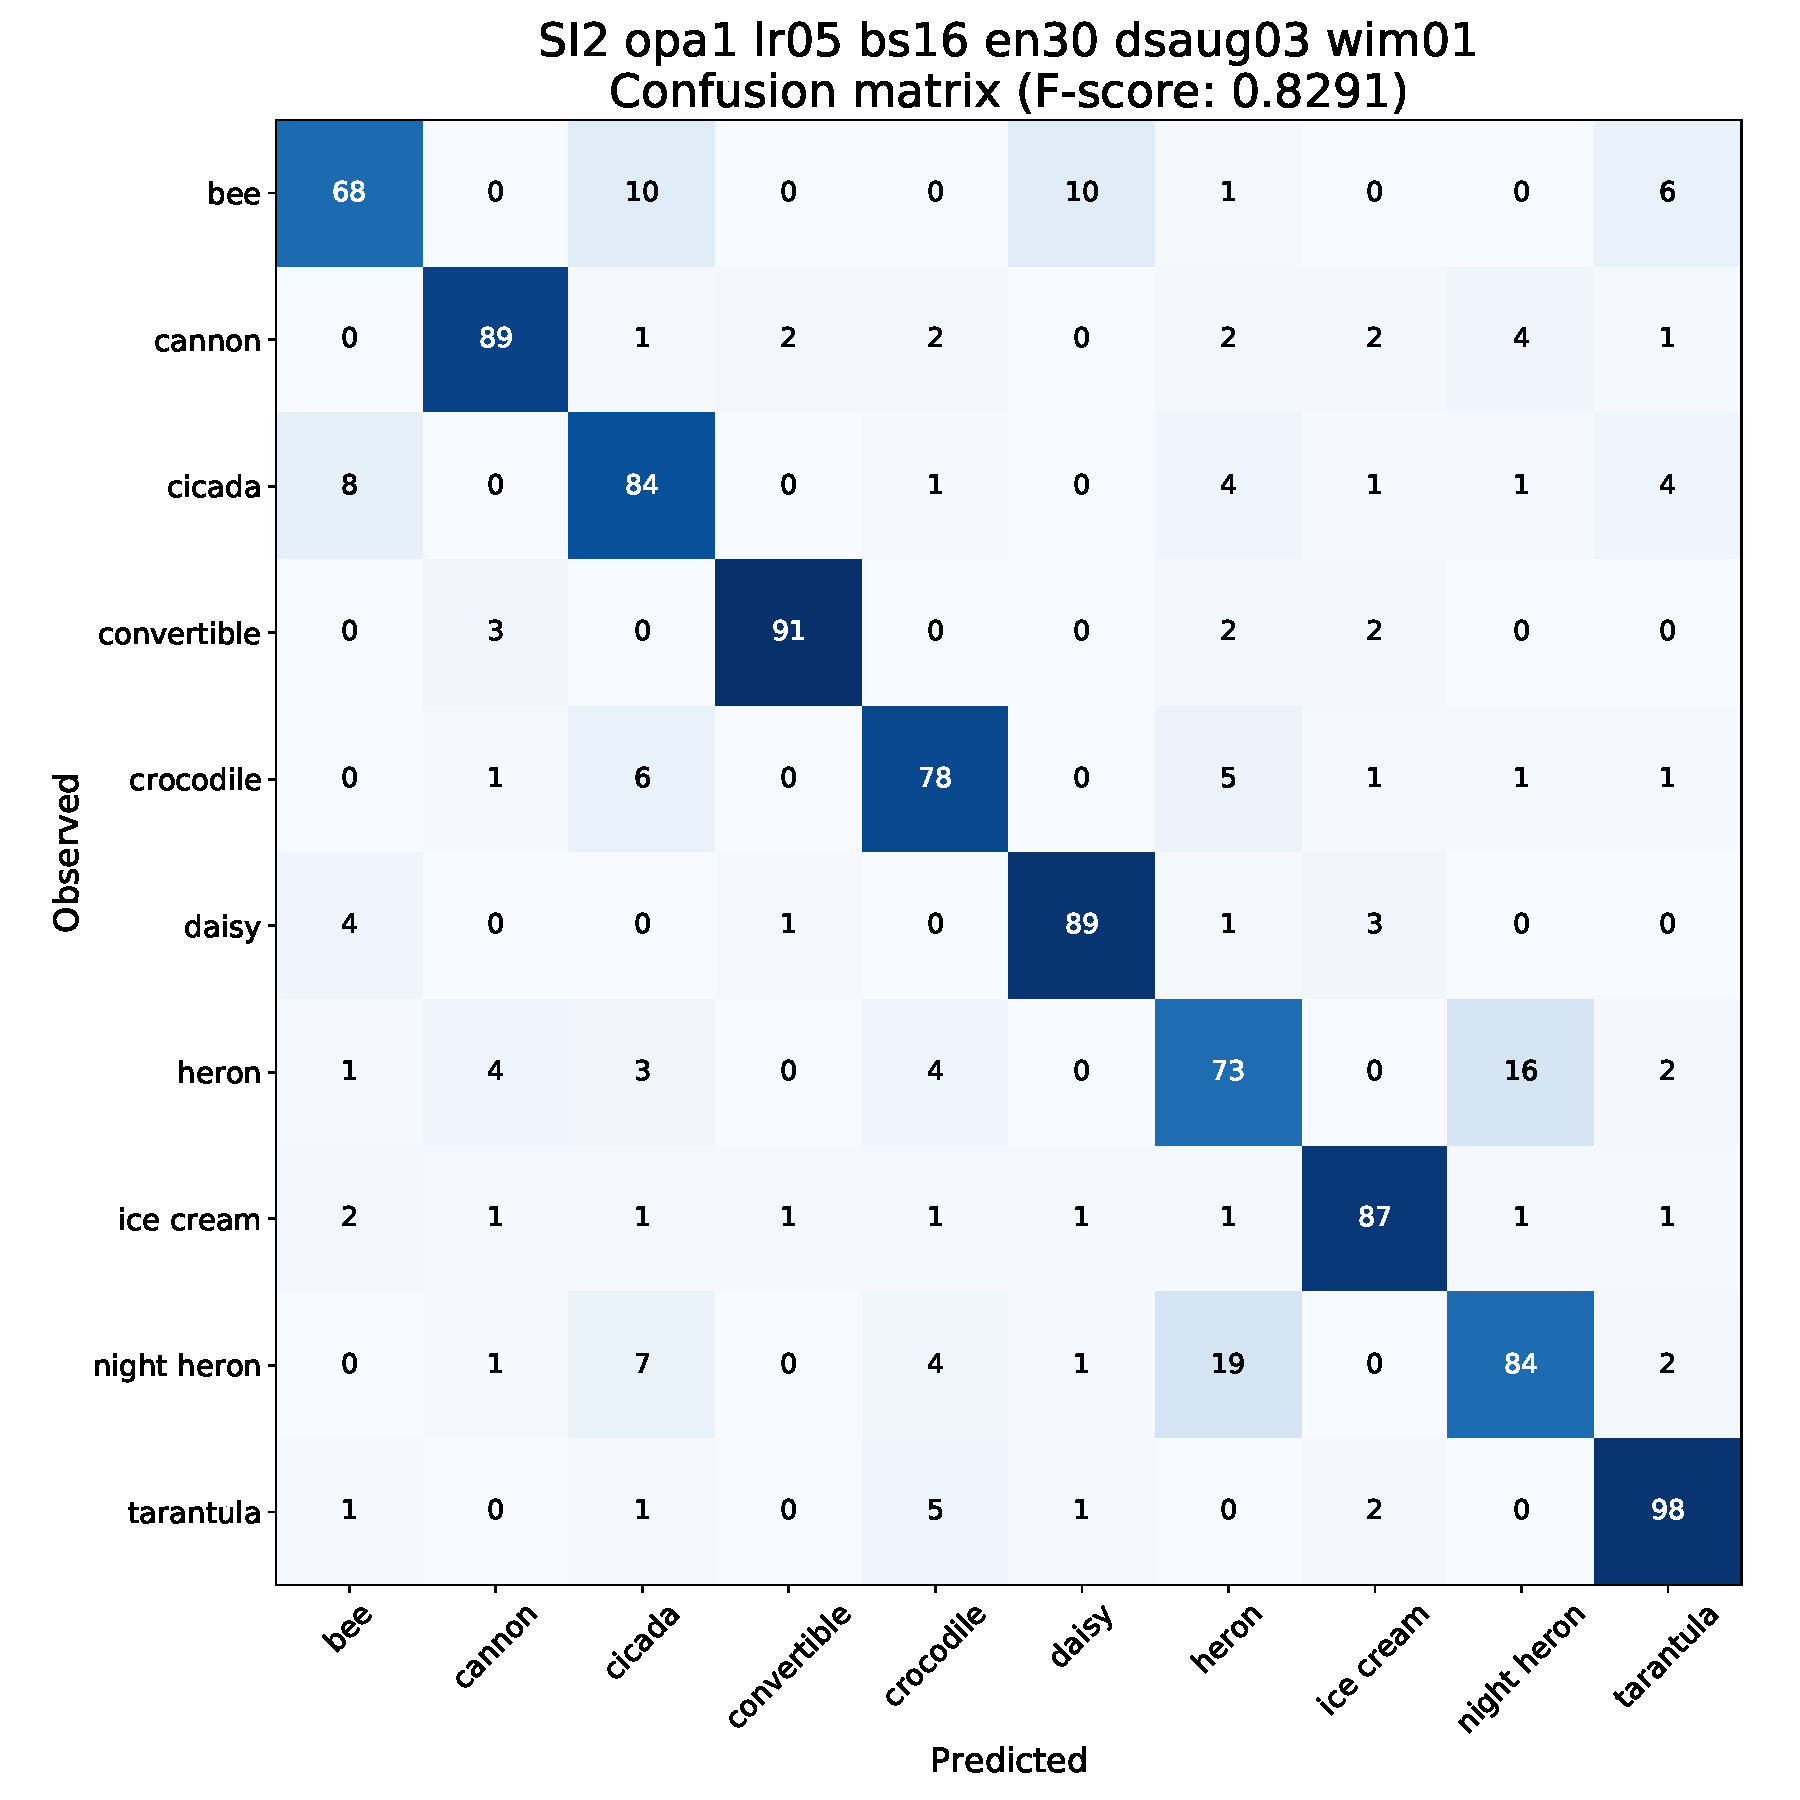
\includegraphics[width=0.8\linewidth]{SI2_opa1_lr05_bs16_en30_dsaug03_wim01_cm.pdf}
    \caption{SimpleNet2 experiment on $10$ ImageNet classes of $800$ images.
        Note that the largest mistakes are between ``heron'' and ``night heron'',
        ``cicada'' and ``bee'', ``daisy'' and ``bee'':
        image classes that are indeed very similar.
    }%
    \label{fig:heron}
\end{figure*}
